\documentclass[mathserif]{beamer}  
 %%%=====For Chinese=====%%%
\usepackage{pptgeshi}  

%%%=====显示指令=====%%%
%\beamerdefaultoverlayspecification{<+->} %使用该命令,许多环境都会自动逐段显示


%%%=====标题信息=====%%%
\title
{第二章 \qquad 数列极限}
\author{}
\date{\sihao \S 3\qquad 数列极限存在的条件}

%%%=====内容=====%%%
\begin{document}
	
%%%=============公式和文字之间的间距
\setlength\abovedisplayskip{2pt}
\setlength\belowdisplayskip{2pt}

%%%%%%%%%%%%%%%%%%%%%%%%%%%%%%%%%%%%%%%%标题
\begin{frame}
\Background
\titlepage  %标题页
\end{frame}




\section{\S 3  数列极限存在的条件}


\begin{frame}
\frametitle{问题:}
\begin{itemize}
\item 怎么知道一个数列是收敛的?即极限的存在性问题;
\jiange
\item 之前的方法:定义.\\
\suojin 需要知道极限;\\
\suojin 具体的证明可能会很麻烦.
\item 其他方法:迫敛性、四则运算.
\item 寻找数列本身特征.
\end{itemize}
\end{frame}


%%%%%%%%%%%%%%%%%%%%%%%%%%%%%%%%%%%%%%%%%%%目录
\begin{frame}
\tableofcontents
\end{frame}



%%%%%%%%%%%%%%%%%%%%%%%%%%%%%%%%%%%%%%%%%%% 单调数列

\subsection{单调数列}
\begin{frame}
\frametitle{单调数列}
\begin{dfn}
\suojin 若数列$a_n$满足:对于$\forall x\in\mathbb{N}_{+}$
$$a_n\leqslant a_{n+1}\ (a_n\geqslant a_{n+1}\ ),$$
则称数列$a_n$为递增(递减)数列.\\
\suojin 单调递增数列与单调递减数列统称为单调数列.
\end{dfn}
\begin{itemize}
\item 类似,可以定义严格单调数列.
\item 与单调函数的定义是统一的.
\item 判断:$\ff{n}{n+1}$、$n^{2}$、$\ff{(-1)^{n}}{n}$\jh
\end{itemize}
\end{frame}




%%%%%%%%%%%%%%%%%%%%%%%--------------------   单调有界定理   ----------------%
\subsection{单调有界定理}

\begin{frame}[label=dandiaoyoujie]
\frametitle{单调有界定理 }
\begin{thm}
\suojin 在实数系中,有界的单调数列必有极限.
\end{thm}
\hfill\hyperlink{dandiaoyoujiezm<1>}{\beamergotobutton{证明过程}}
\begin{itemize}
\item[注1.\ ] 单增有上界的数列极限存在,为其上确界.
\item[注2.\ ] 单减有下界的数列极限存在,为其下确界.
\item[注3.\ ] 单增无上界(单减无下界)的数列$\{a_n\}$有$$\lim_{n\rightarrow\infty}a_{n}=+\infty\quad (\lim_{n\rightarrow\infty}a_{n}=-\infty).$$
\end{itemize}
\end{frame}




%%%%%%%%%%%%%%%%%%%%%%%--------------------   单调有界定理例题   ----------------%
\subsection{单调有界定理例题}
\begin{frame}[label=li_1]
\frametitle{单调有界定理例题}
\begin{ex}
\suojin $\alpha\geqslant 2$,设$$a_{n}=1+\ff{1}{2^{\alpha}}+\cdots+\ff{1}{n^{\alpha}}\jh$$ 证明:$\{a_{n}\}$收敛\jh
\end{ex}
\hfill \hyperlink{li_1jd<1>}{\beamergotobutton{证明过程}}
\end{frame}



\begin{frame}[label=li_2]
\frametitle{单调有界定理例题}
\begin{ex}{\xiaowuhao
\suojin 证明数列
$$\sqrt{2},\ \sqrt{2+\sqrt{2}},\ \sqrt{2+\sqrt{2+\sqrt{2}}},\ \cdots,\ \sqrt{2+\sqrt{2+\cdots+\sqrt{2}}},\ \cdots\ $$
收敛,并求其极限\jh}
\end{ex}
\hfill  \hyperlink{li_2jd<1>}{\beamergotobutton{证明过程}}
\begin{itemize}
\item[注1.\ ] 此类问题一般使用数学归纳法.
\item[注2.\ ] 如何快速找到“界”?.
\end{itemize}
\end{frame}



\begin{frame}
	\frametitle{例题}
		\begin{ex}
		\suojin 下面的叙述错在哪儿?\\
	\suojin “设 $a_n=2^n,\ n=1,2, \cdots$,\ 则
	$$
	a_{n+1}=2^{n+1}=2 a_n .
	$$
	因为显然有 $a_n>0$,所以 $\left\{a_n\right\}$ 递增\jh 设 $\lim _{n \rightarrow \infty} a_n=A$,从而得出
	$$
	A=2 A \Rightarrow A=0
	$$
	即 $\lim _{n \rightarrow \infty} 2^n=0$."
\end{ex}
\end{frame}


\begin{frame}[label=qjsl]
\frametitle{单调有界定理例题}
\begin{prop}
\suojin 设$S$为有界数集\jh 证明:若$\sup S=a\notin S$,则存在严格递增数列$x_{n}\subset S$,使得
$$\lim_{n\rightarrow\infty}x_n =a.$$
\end{prop}
\hfill\hyperlink{qjslzm<1>}{\beamergotobutton{证明过程}}\\
 \suojin 有界数集的下确界有类似结论.
\end{frame}






\begin{frame}[label=li_4]
\frametitle{单调有界定理例题}  
\begin{ex}[4]
\suojin 证明$$\lim_{n\rightarrow\infty}(1+\ff{1}{n}) ^{n}$$
存在.
\end{ex}
\hfill\hyperlink{li_4jd<1>}{\beamergotobutton{证明过程}}
\begin{itemize}
\item[注1\jh] 定义$$\ee=\lim_{n\rightarrow\infty}(1+\ff{1}{n})^{n}.$$
\item[注2\jh] $\ee$ 为无理数,$\ee\approx 2.718281828459$\jh
\item[注3\jh] 以$\ee$为底的对数称为自然对数,记为$\ln x=\log_{e}x$.
\end{itemize}
\end{frame}



\begin{frame}
\frametitle{从证明过程中我们可以得到:}
\begin{itemize}
\item \suojin\suojin\suojin 数列$\{(1+\ff{1}{n})^{n}\}$严格单增.
\item $$(1+\ff{1}{n})^{n}<e.$$
\item $$(1+\ff{1}{n})^{n}<e<(1+\ff{1}{n})^{n+1}.$$
需要证明:$\{(1+\ff{1}{n})^{n+1}.\}$为严格单减数列.
\item $$\ff{1}{n+1}<\ln x<\ff{1}{n}.$$
\end{itemize}
\end{frame}



\begin{frame}[label=li_bc3]{例题}%%%%
	\begin{ex}
		\suojin 设 $s_n=1+\frac{1}{1 !}+\frac{1}{2 !}+\frac{1}{3 !}+\cdots+\frac{1}{n !},\ n=1,2,\ \cdots$, 证明:
		$$
		\lim _{n \rightarrow \infty} s_n=\ee .
		$$ 
	\end{ex}
\jiange

\suojin  利用上例题证明过程中的结果.\\
\hfill\hyperlink{li_bc3jd<1>}{\beamergotobutton{证明过程}}
\end{frame}


\begin{frame}{例题注释}%%%%
	\suojin 由公式 $\mathrm{e}=\lim _{n \rightarrow \infty}\left(1+\frac{1}{1 !}+\frac{1}{2 !}+\frac{1}{3 !}+\cdots+\frac{1}{n !}\right)$,可以较快地算出 \liang{$\mathrm{e}$ 的近似值}.  \\
	\suojin 由于
	$$
	0<s_{n+m}-s_n=\frac{1}{(n+1) !}+\frac{1}{(n+2) !}+\cdots+\frac{1}{(n+m) !},
	$$
	令 $m \rightarrow \infty$, 得到
	$$
	0<e-s_n \leq \frac{1}{n ! n}, n=1,2, \cdots .
	$$
	\suojin 取 $n=10$,$\mathrm{e} \approx s_{10} \approx 2.7182818$,其误差
	$$
	0<\mathrm{e}-s_{10} \leqslant \frac{1}{10 \cdot 10 !}<10^{-7}.
	$$
\end{frame}







\begin{frame}[label=li_bc]
\frametitle{单调有界定理例题}
\begin{ex}
\suojin 设数列$$c_{n}=1+\ff{1}{2}+\cdots+\ff{1}{n}-\ln n,$$
证明:数列$\{c_{n}\}$收敛,并求
$$\lim_{n\rightarrow\infty}\big(\ff{1}{n+1}+\ff{1}{n+2}+\cdots+\ff{1}{2n}\big).$$
\end{ex}
\suojin 注:利用$$\ff{1}{n+1}<\ln (1+\ff{1}{n})<\ff{1}{n}.$$
\hfill \hyperlink{li_bcjd<1>}{\beamergotobutton{证明过程}}
\end{frame}




\begin{frame}[label=li_5]
\frametitle{单调有界定理例题}
\begin{ex}[5]
\suojin 任何数列都存在单调子列.
\end{ex}

\suojin 将数列分为两类:
\begin{itemize}
\item 有单减子列:$\forall k\in\mathbb{N}_{+}$,$\{a_{n+k}\}$有最大项;
\item 有单增子列:存在$k\in\mathbb{N}_{+}$,$\{a_{n+k}\}$无最大项.
\end{itemize}

\hfill\hyperlink{li_5jd<1>}{\beamergotobutton{证明过程}}
\end{frame}




%--------------------   致密性定理   ----------------%
\subsection{致密性定理}

\begin{frame}[label=zmx]
\frametitle{致密性定理}
\begin{thm}
\suojin 任何有界数列必定有收敛子列\jh
\end{thm}
\begin{itemize}
\item[注1\jh] 单调有界定理和例5的直接推论.
\item[注2\jh] 与Weierstrass定理(第七章)等价.
\end{itemize}
\end{frame}


\begin{frame}[label=li_6]
\frametitle{致密性定理例题}
\begin{ex}
\suojin 设数列$\{a_{n}\}$无上界,则存在$\{a_{n}\}$的子列$\{a_{n_k}\}$,
$$\lim_{k\rightarrow\infty}a_{n_k}=+\infty.$$
\end{ex}
\hfill\hyperlink{li_6jd<1>}{\beamergotobutton{证明过程}}
\begin{itemize}
\item[注1\jh] 无下界有类似结论.
\item[注2\jh] 证明中构造子列的方法是常用技巧.
\end{itemize}
\end{frame}




%%%%%%%%%%%%%%%%%%%%%%%--------------------   Cauchy收敛准则   ----------------%
\subsection{Cauchy收敛准则}

\begin{frame}[label=Cauchyzz]
\frametitle{Cauchy收敛准则}
\begin{thm}
\suojin 数列$\{a_{n}\}$收敛的充要条件是:
$$\forall \varepsilon >0 ,\ \mbox{存在}N>0,\ \mbox{使得}\forall n,\ m>N\mbox{时,有}|a_n-a_m|<\varepsilon.$$
\end{thm}
\hfill \hyperlink{Cauchyzm<1>}{\beamergotobutton{证明过程}}
\begin{itemize}
\item[注1\jh] 这一充要条件称为Cauchy条件.
\item[注2\jh] 类似定义形式,相对优势:不需要知道极限.
\item[注3\jh] 几何意义:收敛数列各项的值越到后面,彼此越接近.
\end{itemize}
\end{frame}


\begin{frame}
\frametitle{Cauchy收敛准则}
\suojin Cauchy条件等价形式:
\begin{itemize}
\item $\forall \epsilon >0 ,\ \mbox{存在}N>0,\ \mbox{使得}\forall n,\ m>N\mbox{时,有}|a_n-a_m|<\varepsilon.$
\item $\forall \epsilon >0 ,\ \mbox{存在}N>0,\ \mbox{使得}\forall m>n>N\mbox{时,有}|a_n-a_m|<\varepsilon.$
\item $\forall \epsilon >0 ,\ \mbox{存在}N>0,\ \forall n>N,\ \forall p\in\mathbb{N}_{+},\ \mbox{有}|a_{n+p}-a_n|<\varepsilon.$
\end{itemize}
\jiange
\suojin 逆否命题:
\begin{thm}
\suojin 数列$\{a_{n}\}$发散的充要条件是:存在$\varepsilon_{0} >0$ ,$\forall N>0$,存在$n_{0}>N$,$ p_{0}\in \mathbb{N}_{+}$时,有\quad $|a_n-a_m|\geqslant\varepsilon_{0}.$
\end{thm}
\end{frame}



\subsection{Cauchy收敛准则例题}

\begin{frame}[label=li_7]
\frametitle{Cauchy收敛准则例题}
\begin{ex}
\suojin 证明:任意无限十进制小数
$$\alpha=0.b_{1}b_{2}\cdots b_{n}\cdots$$
的$n(\in\mathbb{N}_{+})$位不足近似
$$\ff{b_{1}}{10},\ \ff{b_{1}}{10}+\ff{b_{2}}{10^{2}},\ \cdots \ff{b_{1}}{10}+\ff{b_{2}}{10^{2}}+\cdots+\ff{b_{n}}{10^{n}},\cdots$$
满足Cauchy条件,其中$b_{k}\in\{0,\ 1,\ 2,\ \cdots ,\ 9\}$,$k\in\mathbb{N}_{+}$\jh
\end{ex}
\hfill\hyperlink{li_7jd<1>}{\beamergotobutton{证明过程}}
 \end{frame}


\begin{frame}
	\frametitle{例题注释}
	\suojin 循环小数 $0 . \dot{9}$ 的不足近似值组成的数列为
	$$
	a_n=\frac{9}{10}+\frac{9}{10^2}+\cdots+\frac{9}{10^n}, \quad n=1,2, \cdots .
	$$
	\suojin 利用等比数列求和公式,可知 
	$$\lim _{n \rightarrow \infty} a_n=\lim _{n \rightarrow \infty} \frac{9}{10} \cdot \frac{1-\left(\frac{1}{10}\right)^n}{1-\frac{1}{10}}=1.$$ 
	这就是为什么可以将无限小数 $0 . \dot{9}$ 表示为 1 的一个原因.
\end{frame}





\begin{frame}{例题}%%%%
\begin{ex}
	\suojin 设 $x_n=1+\frac{1}{3}+\cdots+\frac{1}{n}, n=1,2, \cdots$. 证明 $\left\{x_n\right\}$ 发散.
\end{ex}
\pause
\begin{proofs}
	\suojin  取 $\varepsilon_0=\frac{1}{2},\ \forall N>0,\ \exists n_0=N, m_0=2 N$,使得
	$$
	\begin{aligned}
		\left|x_{n_0}-x_{m_0}\right| & =\frac{1}{N+1}+\frac{1}{N+2}+\cdots+\frac{1}{2 N} \\
		& \geq \frac{1}{2 N}+\frac{1}{2 N}+\cdots+\frac{1}{2 N} \geq \varepsilon_0 .
	\end{aligned}
	$$
	\suojin 由柯西收敛准则的否定陈述,可知 $\left\{x_n\right\}$ 发散. 
\end{proofs}   
\end{frame}




\begin{frame}{例题}%%%%
\begin{ex}
	\suojin 设 $x_n=\frac{\sin 1}{2^1}+\frac{\sin 2}{2^2}+\cdots+\frac{\sin n}{2^n},\ n=1,2, \cdots$.\ 求证 $\left\{x_n\right\}$ 收敛.  
\end{ex}
\pause
\begin{proofs}
	\suojin $\forall \varepsilon>0, \exists N=\frac{-\log \varepsilon}{\log 2}$, 当 $n>m>N$ 时, 有
	$$
	\begin{aligned}
		\mid x_n- & x_m|=| \frac{\sin (m+1)}{2^{m+1}}+\cdots+\frac{\sin n}{2^n} \mid \\
		& \leq \frac{1}{2^{m+1}}+\cdots+\frac{1}{2^n}=\frac{1}{2^{m+1}}\left(1+\frac{1}{2}+\cdots+\frac{1}{2^{n-m-1}}\right) \\
		& =\frac{2}{2^{m+1}}\left(1-\frac{1}{2^{n-m}}\right) \leq \frac{1}{2^m}<\varepsilon \Rightarrow\left\{x_n\right\} \text { 收敛. }
	\end{aligned}
	$$ 
\end{proofs}
\end{frame}




\begin{frame}[label=li_bc2]
\frametitle{Cauchy收敛准则例题}
\begin{ex}
\suojin 设$a_{n}=1+\ff{1}{2^{\alpha}}+\cdots+\ff{1}{n^{\alpha}}$\jh 证明:
\begin{itemize}
\item[(1)\ ] 当$\alpha>1$时,$a_{n}$收敛;
\item[(2)\ ] 当$\alpha\leqslant 1$时,$a_{n}$发散\jh
\end{itemize}
\end{ex}
%\hfill\hyperlink{li_bc2jd<1>}{\beamergotobutton{证明过程}}
\jiange
	\begin{ex}
	\suojin 设数列满足条件:$\left|a_{n+1}-a_n\right|<r^n, n=1,2, \cdots$, 其中 $r \in(0,1)$.\ 求证: $\left\{a_n\right\}$收敛.
	\end{ex}
\hfill\hyperlink{li_bc4jd<1>}{\beamergotobutton{证明过程}}
\end{frame}





\begin{frame}{注释}%%%%
	\begin{alertblock}{}
	\suojin \liang{柯西收敛准则的意义在于:}\\
	\suojin 可以根据数列通项本身的特征来判断该数列是否收敛,而不必依赖于极限定义中的那个极限值 $A$.\ 这一特点在理论上特别有用,大家将会逐渐体会到它的重要性.
	\end{alertblock}
\end{frame}



\begin{frame}{复习思考题}%%%%
	\begin{itemize}
		\item[1.\ ] 对于数列是否收敛的各种判别法加以总结.
		\item[2.\ ] 试给出 $\left\{a_n\right\}$ 不是Cauchy列的正面陈述.
	\end{itemize}
\end{frame}



%%%%%%%%%%%%%%%%%%%%%%%-----------------------------作业
\subsection*{作业}

\begin{frame}
\frametitle{作业:}
\begin{itemize}
	\item P37\quad 习题2.3
	\item[]
	\begin{center}1,3\ (1),5\ (1),7.\end{center}
	\item[]
	\item P39\quad 总练习题
	\item[]
	\begin{center}4,5,6.\end{center}
\end{itemize}
\end{frame}



%%%%%%%%%%%%%%%%%%%%%%%%%%%%%%%%%%%%%%定理和例题的证明过程
\subsection*{定理和例题的证明过程}
%---------------------   单调有界定理的证明   ---------------------%
\begin{frame}[label=dandiaoyoujiezm]
\frametitle{单调有界定理\hfill\hyperlink{dandiaoyoujie<1>}{\beamergotobutton{返回定理}}}
\begin{proofs}
	\suojin 不妨设 $\left\{a_n\right\}$ 单调增,有上界. 由确界定理,存在 
	$$\sup \left\{a_n\right\}=\xi\jh$$  
	\suojin 由上确界的定义,对于任意的 $\varepsilon>0$,存在 $a_{n_0}$,使 $a_{n_0}>\xi-\varepsilon$\jh  故当 $n>n_0(=N)$ 时,
	\begin{center}
		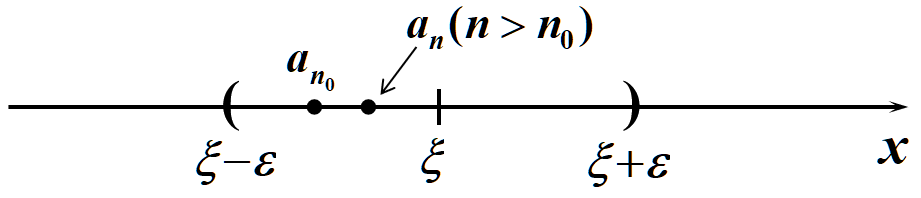
\includegraphics[width=0.5\textwidth]{figures/ddyoujie1.png}
	\end{center}
	$$
	\xi-\varepsilon<a_{n_0} \leq a_n \leq \xi<\xi+\varepsilon,
	$$
	这就证明了 $\lim _{n \rightarrow \infty} a_n=\xi$.
\end{proofs}
\end{frame}





%---------------------   例题1的证明   ---------------------%
\begin{frame}[label=li_1jd]
  \frametitle{例题解答\hfill\hyperlink{li_1<1>}{\beamergotobutton{返回命题}}}
  \begin{proofs}
  \suojin 显然数列$\{a_n\}$单调递增\jh 下面只需要证明数列 $\{a_n\}$ 有界.\\
  \suojin  任意的$n\in \N$,有
  $$
  \begin{aligned}
  	|a_n|&=\left| \frac{1}{1^{\alpha}}+\frac{1}{2^{\alpha}}+\cdots+\frac{1}{n^{\alpha}} \right| \\
  	& \leqslant \frac{1}{1^{2}}+\frac{1}{2^{2}}+\cdots+\frac{1}{n^{2}} \\
  	& \leqslant \frac{1}{1\cdot 2}+\frac{1}{2\cdot 3}+\cdots+\frac{1}{(n-1)\cdot n} \\
  	& =1-\frac{1}{n}<1. \\
  	\Rightarrow&\left\{a_n\right\} \text { 有界,从而收敛. }
  \end{aligned}
  $$ 
  \end{proofs} 
\end{frame}




%---------------------   例题2的证明   ---------------------%
\begin{frame}[label=li_2jd]{例题解答\hfill  \hyperlink{li_2<1>}{\beamergotobutton{返回例题}}}%%%%
	\begin{jie}
		\suojin 记上述数列为
		$$a_{1}=\sqrt{2},\ a_{2}=\sqrt{2+\sqrt{2}},\ \cdots,\ a_{n}=\sqrt{2+\sqrt{2+\cdots+\sqrt{2}}},\ \cdots\ $$
		\suojin 显然$a_n>0$\jh 因 $a_2=\sqrt{2+\sqrt{2}}$,故 $a_2>a_1$;\\
		\suojin 设 $a_n>a_{n-1}$,则有
		$$
		\begin{aligned}
			a_{n+1}-a_n & =\sqrt{2+a_n}-\sqrt{2+a_{n-1}} \\
			& =\frac{a_n-a_{n-1}}{\sqrt{2+a_n}+\sqrt{2+a_{n-1}}}>0,
		\end{aligned}
		$$
		所以 $\left\{a_n\right\}$ 递增\jh 下面再来证明此数列有上界.
	\end{jie}
\end{frame}




\begin{frame}{例题解答\hfill  \hyperlink{li_2<1>}{\beamergotobutton{返回例题}}}%%%%
	\begin{proofs}
		\suojin 显然,$a_1=\sqrt{2}<2$,设 $a_n<2$,则
		$$
		a_{n+1}=\sqrt{2+a_n}<\sqrt{2+2}=2 .
		$$
		由此得到 $\left\{a_n\right\}$ 有上界 2,故极限 $\lim _{n \rightarrow \infty} a_n=A$ 存在.\\ \xiaojg
	\suojin 于是由 $\lim _{n \rightarrow \infty} a_{n+1}=\lim _{n \rightarrow \infty} \sqrt{2+a_n}$, 可得
	$$A^2=2+A,$$ 
	并解出 $A=2,\ A=-1$.\\
	\suojin 由极限的不等式性, 知道 $A>0$, 所以
	$$
	\lim _{n \rightarrow \infty} a_n=2.
	$$  
    \end{proofs}
\end{frame}



%-------------------   例题4的证明e   ----------------------------%


\begin{frame}[label=li_4jd]{例题证明\hfill\hyperlink{li_4<1>}{\beamergotobutton{返回例题}}}%%%%
	\suojin 考察数列 $\left\{e_n\right\}=\left\{\left(1+\frac{1}{n}\right)^n\right\}$ 的收敛性,下面的证法是最基本的,而教材上的证法技巧性较强.
	\begin{proofs}
		\suojin 利用二项式展开,得
		{\xiaowuhao
			$$
			\begin{aligned}
				e_n= & 1+n \frac{1}{n}+\frac{n(n-1)}{2 !} \frac{1}{n^2}+\cdots+\frac{n(n-1) \cdots 1}{n !} \frac{1}{n^n} \\
				= & +\frac{1}{1 !}+\frac{1}{2 !}\left(1-\frac{1}{n}\right)+\frac{1}{3 !}\left(1-\frac{1}{n}\right)\left(1-\frac{2}{n}\right) \\
				& +\cdots+\frac{1}{n !}\left(1-\frac{1}{n}\right)\left(1-\frac{2}{n}\right) \cdots\left(1-\frac{n-1}{n}\right),
			\end{aligned}
			$$}
	\end{proofs}
\end{frame}




\begin{frame}{例题证明\hfill\hyperlink{li_4<1>}{\beamergotobutton{返回例题}}}%%%%
	\begin{proofs}
		由此得{\xiaowuhao
			$$
			\begin{aligned}
				e_{n+1}=1 & +\frac{1}{1 !}+\frac{1}{2 !}\left(1-\frac{1}{n+1}\right)+\frac{1}{3 !}\left(1-\frac{1}{n+1}\right)\left(1-\frac{2}{n+1}\right) \\
				& +\cdots+\frac{1}{n !}\left(1-\frac{1}{n+1}\right)\left(1-\frac{2}{n+1}\right) \cdots\left(1-\frac{n-1}{n+1}\right) \\
				& +\frac{1}{(n+1) !}\left(1-\frac{1}{n+1}\right)\left(1-\frac{2}{n+1}\right) \cdots\left(1-\frac{n}{n+1}\right) .
			\end{aligned}
			$$}
		\suojin 把 $e_n$ 和 $e_{n+1}$ 的展开式作比较就可发现,$e_n$ 的展开式有 $n+1$ 项,其中的每一项都比 $e_{n+1}$ 的展开式中的前 $n+1$ 项小,而 $e_{n+1}$ 的最后一项大于零. 
	\end{proofs}
	
\end{frame}




\begin{frame}{例题证明\hfill\hyperlink{li_4<1>}{\beamergotobutton{返回例题}}}%%%%
	\begin{proofs}
		\suojin 因此  
		$$
		e_n<e_{n+1}, \quad n=1,2, \cdots,
		$$
		从而 $\left\{\mathrm{e}_n\right\}$ 是单调增数列,且
		$$
		e_n \leq 1+\frac{1}{1 !}+\frac{1}{2 !}+\frac{1}{3 !}+\cdots+\frac{1}{n !} .
		$$
		由此 $e_n \leq 1+1+\frac{1}{2}+\frac{1}{2^2}+\cdots+\frac{1}{2^{n-1}}<3$,这就证明了 $\left\{e_n\right\}$ 又是有界数列\jh 于是 $\lim _{n \rightarrow \infty} e_n$ 存在\jh 记此极限为 $\ee$,即
		\liang{
			$$
			\mathrm{e}=\lim _{n \rightarrow \infty}\left(1+\frac{1}{n}\right)^n.
			$$ } 
	\end{proofs}
\end{frame}






%------------------------  例题5的证明   --------------------------%

\begin{frame}[label=li_5jd]
	\frametitle{例题解答\hfill \hyperlink{li_5<1>}{\beamergotobutton{返回例题}}}
	\begin{proofs}
		\suojin 设数列为$\{a_{n}\}$\jh 下面分两种情形来讨论.\\
		\suojin \liang{1.\ } 对于任意的$k\in\mathbb{N}_{+}$,数列$\{a_{n+k}\}$有最大项\jh \\
		\suojin 设$\{a_{1+n}\}$的最大项为 $\{a_{n_1}\}$,因为 $\{a_{n_{1}+n}\}$ 也有最大项,设其最大项为 $\{a_{n_2}\}$,显然有$n_{2}>n_{1}$,且因 $\{a_{n_{1}+n}\}$ 是 $\{a_{1+n}\}$ 的一个子列,故$a_{n_{2}}\leqslant a_{n_{1}}$;\\
		\suojin 同理存在$n_{3}>n_{2}$,使得$a_{n_{3}}\leqslant a_{n_{2}}$;\\
		\suojin $\cdots\cdots$\\
		\suojin 这样就得到一个单调递减的子列$\{a_{n_k}\}$.
	\end{proofs}
\end{frame}



\begin{frame}
	\frametitle{例题解答\hfill \hyperlink{li_5<1>}{\beamergotobutton{返回例题}}}
	\begin{proofs}
		\suojin \liang{2.\ } 至少存在某正整数$k$,数列$\{a_{n+k}\}$没有最大项\jh \\
		\suojin 先取$n_{1}=k+1$,因为$\{a_{k+n}\}$没有最大项,故 $\{a_{n_{1}}\}$ 后面总存在$\{a_{n_{2}}\}(n_{2}>n_{1})$,使得$$a_{n_{2}}>a_{n_{1}};$$
		\suojin 同理存在$a_{n_{2}}$后面的项$\{a_{n_{3}}\}(n_{3}>n_{2})$,使得$$a_{n_{3}}>a_{n_{2}};$$
		\suojin $\cdots\cdots$\\
		\suojin 这样就得到一个严格递增的子列$\{a_{n_k}\}$.
	\end{proofs}
\end{frame}





%------------------------  例题6的证明   --------------------------%

\begin{frame}[label=li_6jd]
	\frametitle{例题解答\hfill \hyperlink{li_6<1>}{\beamergotobutton{返回例题}}}
	\begin{proofs}
		\suojin 因为 $\left\{a_n\right\}$ 无上界,所以对于任意正数 $M$,存在 $a_{n_0}$,使得 $a_{n_0}>M$. \\
		\suojin 据此分别取 \\
		\suojin $M_1=1$,存在 $a_{n_1}, a_{n_1}>1$;\\
		\suojin $M_2=\max \left\{2,\left|a_1\right|,\left|a_2\right|, \cdots,\left|a_{n_1}\right|\right\}$,存在 
		$$a_{n_2}\left(n_2>n_1\right)\text{,使得} a_{n_2}>M_2;$$
		\suojin $\cdots\cdots$
	\end{proofs}
\end{frame}



\begin{frame}[label=li_6jd]
	\frametitle{例题解答\hfill \hyperlink{li_6<1>}{\beamergotobutton{返回例题}}}
	\begin{proofs}
		\suojin $M_k=\max \left\{k,\left|a_1\right|,\left|a_2\right|, \cdots,\ \left|a_{n_{k-1}}\right|\right\}$,存在 
		$$a_{n_k}\left(n_k>n_{k-1}\right)\text{,使得} a_{n_k}>M_k;$$
		\suojin $\cdots\cdots$\\
		\suojin 由此得到 $\left\{a_n\right\}$ 的一个子列 $\left\{a_{n_k}\right\}$, 满足 $a_{n_k}>M_k \geqslant k$, 推得
		$$
		\lim _{k \rightarrow \infty} a_{n_k}=+\infty .
		$$
	\end{proofs}
\end{frame}





%------------------------  例题7的证明   --------------------------%

\begin{frame}[label=li_7jd]
\frametitle{例题解答\hfill \hyperlink{li_7<1>}{\beamergotobutton{返回例题}}}
\begin{proofs}
	\suojin 记 $a_n=\frac{b_1}{10}+\frac{b_2}{10^2}+\cdots+\frac{b_n}{10^n}$. 不妨设 $n>m$, 则有
	$$
	\begin{aligned}
		\left|a_n-a_m\right| & =\frac{b_{m+1}}{10^{m+1}}+\frac{b_{m+2}}{10^{m+2}}+\cdots+\frac{b_n}{10^n} \\
		& \leqslant \frac{9}{10^{m+1}}\left(1+\frac{1}{10}+\cdots+\frac{1}{10^{n-m-1}}\right) \\
		& =\frac{1}{10^m}\left(1-\frac{1}{10^{n-m}}\right)<\frac{1}{10^m}<\frac{1}{m} .
	\end{aligned}
	$$
	对任给的 $\varepsilon>0$, 取 $N=\frac{1}{\varepsilon}$, 则对一切 $n>m>N$, 有
	$$
	\left|a_n-a_m\right|<\varepsilon .
	$$
	这就证明了数列满足柯西条件.
\end{proofs}
\end{frame}





%-----------------------------      ---------------------------------%




\begin{frame}[label=li_bc3jd]{例题解答\hfill\hyperlink{li_bc3<1>}{\beamergotobutton{返回例题}}}%%%%
	\begin{ex}
		\suojin 设 $s_n=1+\frac{1}{1 !}+\frac{1}{2 !}+\frac{1}{3 !}+\cdots+\frac{1}{n !},\ n=1,2,\ \cdots$, 证明:
		$$
		\lim _{n \rightarrow \infty} s_n=\ee .
		$$ 
	\end{ex}
	\begin{proofs}
		\suojin  显然 $\left\{s_n\right\}$ 是单调增数列, 且由上例证明中可知,
		$$
		\begin{aligned}
			e_n & \leqslant 1+\frac{1}{1 !}+\frac{1}{2 !}+\frac{1}{3 !}+\cdots+\frac{1}{n !} \\
			& =s_n<1+1+\frac{1}{2}+\frac{1}{2^2}+\cdots+\frac{1}{2^{n-1}}<3,
		\end{aligned}
		$$
		因此 $\lim _{n \rightarrow \infty} s_n$ 存在且由极限的保不等式性,
		$$
		\mathrm{e}=\lim _{n \rightarrow \infty} e_n \leqslant \lim _{n \rightarrow \infty} s_n \text {. }
		$$ 
	\end{proofs} 
\end{frame}



\begin{frame}{例题解答\hfill\hyperlink{li_bc3<1>}{\beamergotobutton{返回例题}}}%%%%
	\begin{proofs}
		又对任意 $n>m$ ,
		$$
		\begin{aligned}
			e_n=1 & +\frac{1}{1 !}+\frac{1}{2 !}\left(1-\frac{1}{n}\right)+\frac{1}{3 !}\left(1-\frac{1}{n}\right)\left(1-\frac{2}{n}\right) \\
			& +\cdots+\frac{1}{n !}\left(1-\frac{1}{n}\right)\left(1-\frac{2}{n}\right) \cdots\left(1-\frac{n-1}{n}\right) \\
			>1 & +\frac{1}{1 !}+\frac{1}{2 !}\left(1-\frac{1}{n}\right)+\frac{1}{3 !}\left(1-\frac{1}{n}\right)\left(1-\frac{2}{n}\right) \\
			& +\cdots+\frac{1}{m !}\left(1-\frac{1}{n}\right)\left(1-\frac{2}{n}\right) \cdots\left(1-\frac{m-1}{n}\right),
		\end{aligned}
		$$
	\end{proofs}
\end{frame}



\begin{frame}{例题解答\hfill\hyperlink{li_bc3<1>}{\beamergotobutton{返回例题}}}%%%%
	\begin{proofs}
		因此, 在上式中两边令 $n \rightarrow \infty$, 得
		$$
		\ee=\lim _{n \rightarrow \infty} e_n \geqslant 1+\frac{1}{1 !}+\frac{1}{2 !}+\frac{1}{3 !}+\cdots+\frac{1}{m !}=s_m .
		$$
		\suojin 当 $m \rightarrow \infty$ 时,由极限的保不等式性, 
		$$\mathrm{e} \geqslant \lim _{m \rightarrow \infty} s_m.$$
		从而
		$$
		\mathrm{e}=\lim _{n \rightarrow \infty} s_n=\lim _{n \rightarrow \infty}\left(1+\frac{1}{1 !}+\frac{1}{2 !}+\frac{1}{3 !}+\cdots+\frac{1}{n !}\right) .
		$$
	\end{proofs}		
\end{frame}





%-----------------------------      ---------------------------------%

\begin{frame}[label=qjslzm]{命题的证明\hfill\hyperlink{qjsl<1>}{\beamergotobutton{返回命题}}}%%%%
	\begin{proofs}
		\suojin  因 $a$ 是 $S$ 的上界,故对 $\forall \varepsilon>0,\ \exists x \in S$,使得 $x>a-\varepsilon$.\ 又因 $a \notin S$,故 $x<a$,从而有
		$$
		a-\varepsilon<x<a.
		$$
		现取 $\varepsilon_1=1$,则 $\exists x_1 \in S$,使得
		$$
		a-\varepsilon_1<x_1<a .
		$$
		再取 $\varepsilon_2=\min \left\{\frac{1}{2},\ a-x_1\right\}$,则 $\exists x_2 \in S$,使得  
		$$
		a-\varepsilon_1<x_2<a,
		$$
		且有 $$x_2>a-\varepsilon_2 \geq a-\left(a-x_1\right)=x_1.$$
	\end{proofs}
\end{frame}




\begin{frame}{命题的证明\hfill\hyperlink{qjsl<1>}{\beamergotobutton{返回命题}}}%%%%
	\begin{proofs}
		\suojin 一般地,按上述步骤得到 $\boldsymbol{x}_{n-1}$ 之后,取
		$$
		\varepsilon_n=\min \left\{\frac{1}{n}, a-x_{n-1}\right\},
		$$
		则存在 $x_n \in S$,使得
		$$
		a-\varepsilon_n<\boldsymbol{x}_n<a
		$$
		且有 $x_n>a-\varepsilon_n \geq a-\left(a-x_{n-1}\right)=x_{n-1}$.
		于是得到 $\left\{x_n\right\} \subset S$,它是严格单调的,满足  
		$$
		a-\varepsilon_n<\boldsymbol{x}_n<\boldsymbol{a},
		$$
		因此,$\left|x_n-a\right|<\varepsilon_n \leq \frac{1}{n}, n=1,2, \cdots$.\\
		\suojin 这就证明了 $\lim _{n \rightarrow \infty} x_n=a$.
	\end{proofs}
\end{frame}




%------------------------  补充例题的证明   --------------------------%

\begin{frame}[label=li_bcjd]
\frametitle{例题解答\hfill \hyperlink{li_bc<1>}{\beamergotobutton{返回例题}}}
\begin{proofs}
	$$
	\begin{aligned}
		c_{n+1}-c_{n}=&1+\ff{1}{2}+\cdots+\ff{1}{n}+\ff{1}{n+1}\\
		&-\ln (n+1)-(1+\ff{1}{2}+\cdots+\ff{1}{n}-\ln n)\\
		=&\ff{1}{n+1}-\ln(1+\ff{1}{n})<0.
	\end{aligned}
	$$
	故数列$\{c_{n}\}$单调递减.\\
	\suojin \liang{下面需证数列$\{c_{n}\}$有下界.}
\end{proofs}
\end{frame}




\begin{frame}
\frametitle{例题解答\hfill \hyperlink{li_bc<1>}{\beamergotobutton{返回例题}}}
\begin{proofs}
	\suojin 由例4推得的不等式,有
	$$\begin{aligned}
		\ff{1}{2}<&\ln (1+1)<1,\\
		\ff{1}{3}<&\ln (1+\ff{1}{2})<1,\\
		\cdots,\\
		\ff{1}{n+1}<&\ln (1+\ff{1}{n})<\ff{1}{n}.
	\end{aligned}$$
	综上可得,
	$$\begin{aligned}
		\ff{1}{2}+\ff{1}{3}+\cdots+\ff{1}{n}<&\ln 2+\ln \ff{3}{2}+\ln \ff{4}{3}+\cdots+\ln \ff{n+1}{n}\\
		<&1+\ff{1}{2}+\cdots+\ff{1}{n}.
	\end{aligned}$$
\end{proofs}
\end{frame}



\begin{frame}
\frametitle{例题解答\hfill \hyperlink{li_bc<1>}{\beamergotobutton{返回例题}}}
\begin{proofs}
	\suojin 不等式两边减去 $\ln n$,得到
	$$\begin{aligned}
		&\ff{1}{2}+\ff{1}{3}+\cdots+\ff{1}{n}-\ln n\\
		<&\ln \left(2\cdot \ff{3}{2}\cdot\ff{4}{3}\cdot\ff{n+1}{n}\right)-\ln n\\
		=&\ln(n+1)-\ln n>0.
	\end{aligned}$$
	由单调有界定理可知,数列$\{c_{n}\}$收敛.
\end{proofs}
\end{frame}



\begin{frame}
\frametitle{例题解答\hfill \hyperlink{li_bc<1>}{\beamergotobutton{返回例题}}}
\begin{jie}
	\suojin 设$\lim_{n\rightarrow\infty}c_{n}=c$,故$\lim_{n\rightarrow\infty}c_{2n}=c$\jh 从而有
	$$\begin{aligned}
		&\lim_{n\rightarrow\infty}(c_{2n}-c_{n})\\
		=&\lim_{n\rightarrow\infty}\left(\ff{1}{n+1}+\ff{1}{n+2}+\cdots+\ff{1}{2n}-\ln (2n)+\ln n\right)\\
		=&\lim_{n\rightarrow\infty}\left(\ff{1}{n+1}+\ff{1}{n+2}+\cdots+\ff{1}{2n}-\ln 2\right)\\
		=&0,\\
		\text{所以,}&\lim_{n\rightarrow\infty}\left(\ff{1}{n+1}+\ff{1}{n+2}+\cdots+\ff{1}{2n}\right)=\ln 2.
	\end{aligned}$$
\end{jie}
\end{frame}





%--------------------------   Cauchy收敛准则证明   ---------------------------%


\begin{frame}[label=Cauchyzm]{Cauchy收敛准则的证明 \hfill\hyperlink{Cauchyzz<1>}{\beamergotobutton{证明过程}}}%%%%
	\begin{multicols}{2}
		\suojin \zheng 设 $\lim _{n \rightarrow \infty} a_n=A$.\\
		\suojin 由极限定义,$\forall \varepsilon>0$, $\exists N>0$,当 $n, m>N($ 或 $n, m \geq N)$ 时,有
		$$
		\left|a_n-A\right|<\frac{\varepsilon}{2},\quad \left|a_m-A\right|<\frac{\varepsilon}{2} . 
		$$
		由此推得
		$$
		\begin{aligned}
			&\left|a_n-a_m\right| \leqslant\left|a_n-A\right|+\left|a_m-A\right|\\
			<&\frac{\varepsilon}{2}+\frac{\varepsilon}{2}=\varepsilon .
		\end{aligned}
		$$  
		\begin{center}
			\vspace{-0.85\baselineskip}
			% \renewcommand{\figurename}{图}
			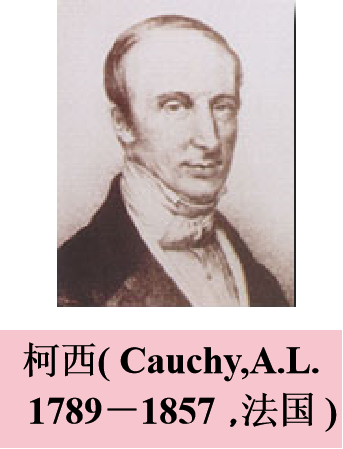
\includegraphics[width=0.3\textwidth]{figures/cauchy.png}
			% \caption{~}
			\vspace{-0.85\baselineskip}
		\end{center}
	\end{multicols}
\end{frame}



%-----------------------------       -------------------------------%



\begin{frame}[label=li_bc4jd]{例题解答\hfill\hyperlink{li_bc2<1>}{\beamergotobutton{返回例题}}}%%%%
	\begin{proofs}
		\suojin  若 $n<m$,则
		$$
		\begin{aligned}
			\left|a_n-a_m\right| & \leq\left|a_n-a_{n+1}\right|+\left|a_{n+1}-a_{n+2}\right|+\cdots+\left|a_{m-1}-a_m\right| \\
			& \leq r^n+r^{n+1}+\cdots+r^{m-1}=\frac{r^n-r^m}{1-r}<\frac{r^n}{1-r} .
		\end{aligned}
		$$
		\suojin 由于 $\lim _{n \rightarrow \infty} \frac{r^n}{1-r}=0$,于是 $\forall \varepsilon>0,\  \exists N,\  n>N$,
		$$
		\left|\frac{r^n}{1-r}\right|<\varepsilon.
		$$   
		若 $m>n>N$,就有
		$$
		\left|a_{n}-a_m\right| \leq\left|\frac{r^n}{1 - r}\right|<\varepsilon .
		$$
		由柯西准则,$\left\{a_n\right\}$ 收敛.
	\end{proofs}
\end{frame}


\end{document} 

